\FloatBarrier

\begin{figure}[h!]
	\centering
	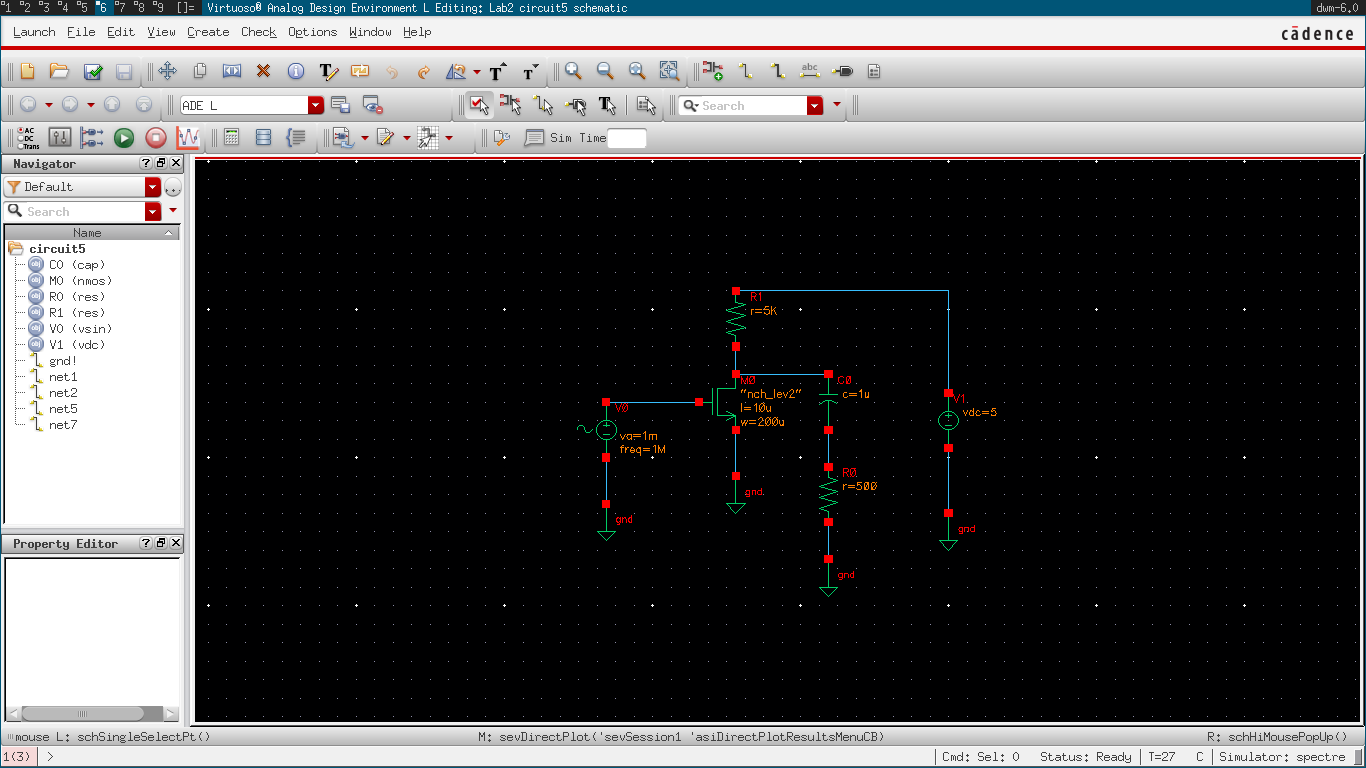
\includegraphics[scale=0.30]{./images/circuit5.PNG}
	\caption{Circuit 5}
	\label{fig:circuit5}
\end{figure}

\FloatBarrier

\FloatBarrier

\begin{figure}[h!]
	\centering
	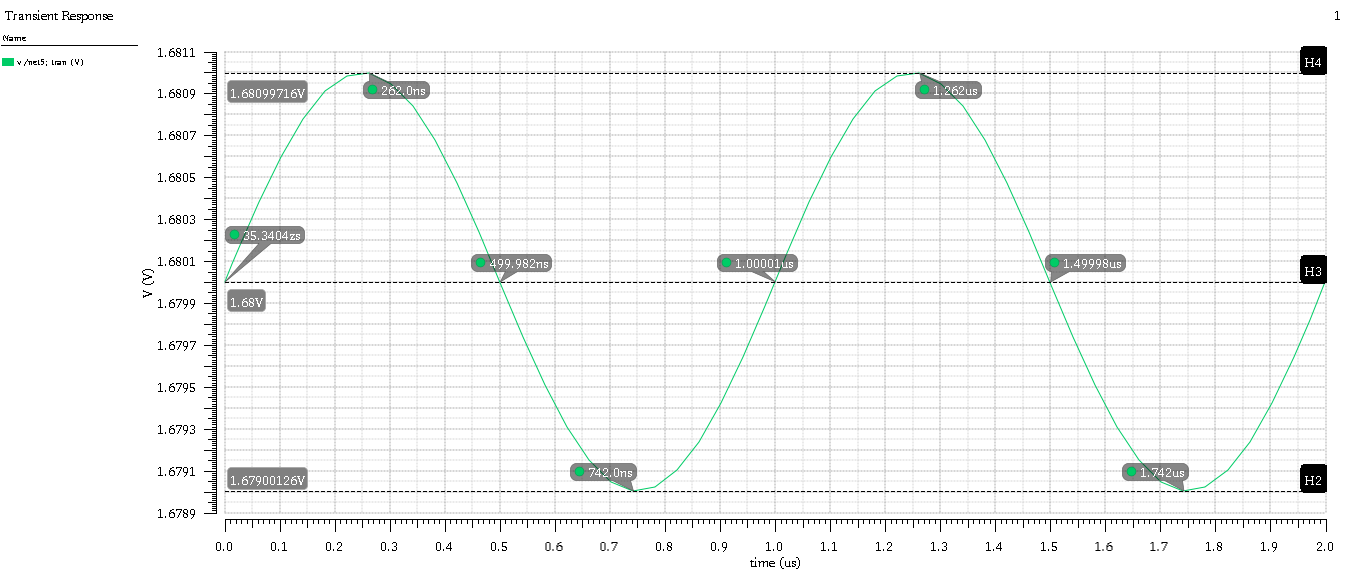
\includegraphics[scale=0.45]{./images/sim5_vin.PNG}
	\caption{$V_{in}$ for Small-Signal Test of Circuit 5}
	\label{fig:sim5_vin}
\end{figure}

\FloatBarrier

\FloatBarrier

\begin{figure}[h!]
	\centering
	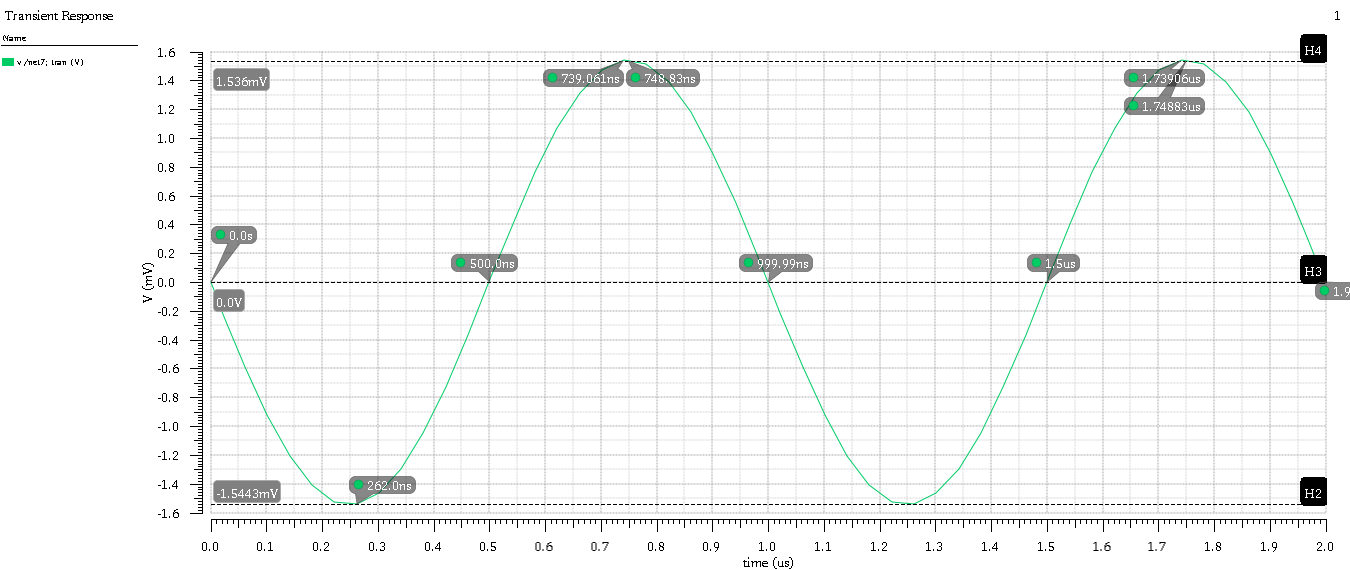
\includegraphics[scale=0.45]{./images/sim5_vout.PNG}
	\caption{$V_{out}$ for Small-Signal Test of Circuit 5}
	\label{fig:sim5_vout}
\end{figure}

\FloatBarrier

The small-signal gain can simply be acquired by taking the ratio of the amplitude of $V_{out}$ to the amplitude of $V_{in}$. This should also be multiplied by a factor of $-1$ since the signals are out of phase by $180^{o}$.
The gain can be determined theoretically from $-g_{m} ( R_{D} || R_{L} || r_{o} )$.
Note that the capacitor at the output eliminates the DC bias voltage and passes an unbiased small signal to the output of the amplifier.

% Determine gain for Circuit 5

\FloatBarrier

\begin{table}[h!]
	\centering
	\caption{Common-Source Amplifier Gain}
	\label{tab:common_source_amp_gain}
	\csvautotabular{./tables/common_source_amp_gain.csv}
\end{table}

\FloatBarrier

% Determine gain for Circuit 6

\FloatBarrier

\begin{figure}[h!]
	\centering
	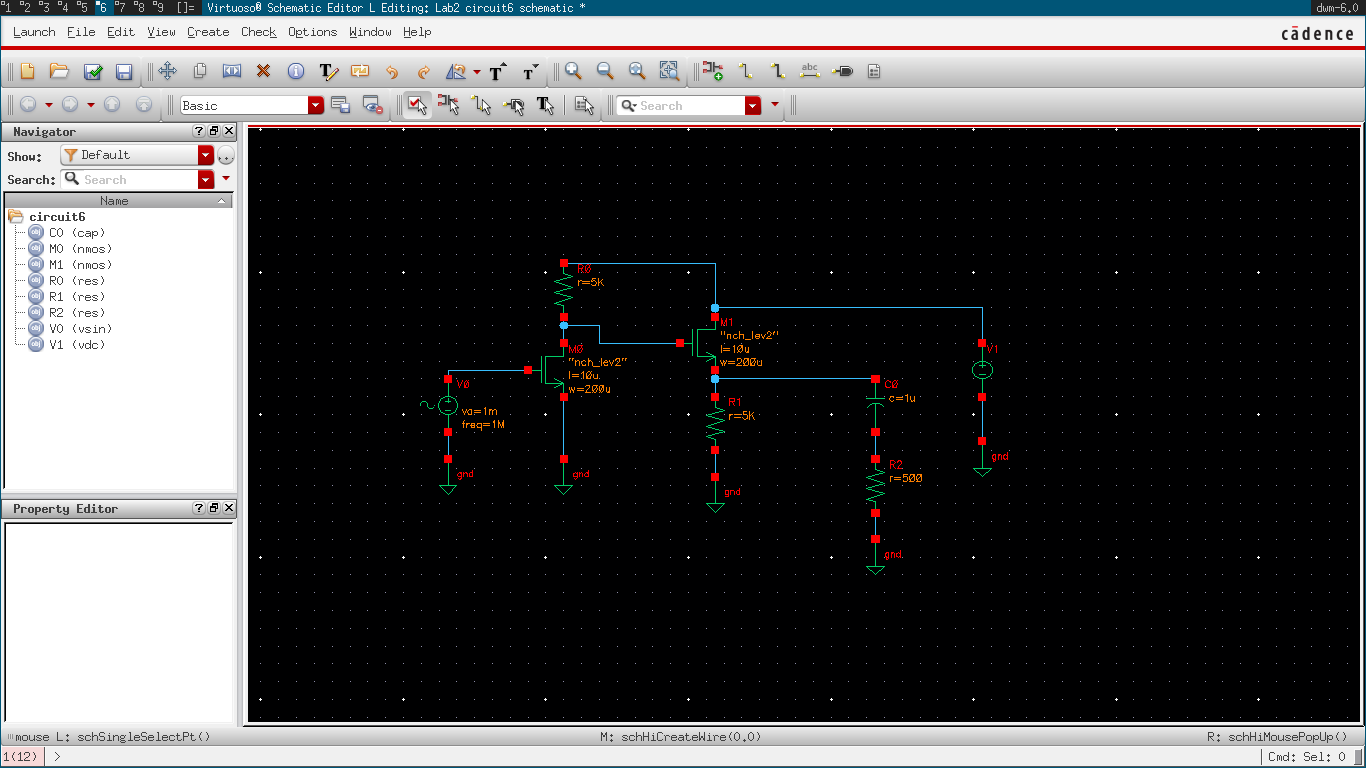
\includegraphics[scale=0.30]{./images/circuit6.PNG}
	\caption{Cascaded Two-Stage Amplifier}
	\label{fig:circuit6}
\end{figure}

\FloatBarrier

The common-drain amplifier at the output will present nearly the same output voltage, but with a much lower output resistance.
The theoretical gain can be calculated by multiplying a common-source gain with a common-drain gain (usually about $1$) and then applying the voltage division equation.

\begin{equation}
	\label{eq:theoretical_cascaded_gain}
	A_{cascade} = \frac{ A_{CSA} A_{CDA} R_{L} }{ r_{out,CDA} + R_{L} }
\end{equation}

\FloatBarrier

\begin{table}[h!]
	\centering
	\caption{Gain of Cascaded Amplifier}
	\label{tab:cascade_gain}
	\csvautotabular{./tables/cascade_gain.csv}
\end{table}

\FloatBarrier

A discrepancy exists between the theoretical value of the cascaded gain and the actual simulation result.
The simulation likely accounts for parameters that are difficult to capture in theoretical calculations, such as the nonideal effects of the decoupling capacitor in the circuit.
What is clear from either result is that the gain of the amplifier increases.
This is because the common-drain amplifier's lower output resistance decreases the significance of the loading effect.
So, instead of the load resistance causing the gain to drop as a result of a voltage divider effect, the load resistance receives a greater portion of the voltage drop because the output resistance of the amplifier has decreased.
